\newlecture

\setcounter{section}{2}
%\def\textbookchapter{Chapter 9: Multivariable and Vector Functions}
\def\coursetopicnumber{I}
\def\textbooksection{9.3} % corresponding textbook section
\def\topic{The Dot Product} % this is the printed title
\def\shorttopic{Dot product} % short topic
\def\textbookname{Active Calculus} % this is the textbook
\def\textbooksectionurl{https://activecalculus.org/vector/S-9-3-Dot-Product.html} % URL for textbook section
\def\handoutday{} % this is the printed date

%%%%%%%%% DOCUMENT CONTENT STARTS BELOW

\thispagestyle{plain}
\topstuff
\section{\topic{} \booklink{}}
\label{sec:dot-product}
The dot product gives us a way to ``multiply'' one vector by another vector. We start with a computational definition, and we will see that it gives us some really useful information about the angle between the vectors.

\subsection{Dot product}
\begin{defn}[Dot product in $\mathbb{R}^2$]
    Suppose $\vec{u}=\langle u_1,u_2\rangle$ and $\vec{v}=\langle v_1,v_2\rangle$ are vectors in $\mathbb{R}^2$.
    
    The \emph{dot product} of $\vec{u}$ and $\vec{v}$ is 
    \[
        \vec{u}\dotp \vec{v}=\langle u_1,u_2\rangle \dotp \langle v_1,v_2\rangle = \hspace{2in}
    \]
\end{defn}

\begin{defn}[Dot product in $\mathbb{R}^3$]
    Suppose $\vec{u}=\langle u_1,u_2,u_3\rangle$ and $\vec{v}=\langle v_1,v_2,v_3\rangle$ are vectors in $\mathbb{R}^3$.
    \bigskip
    
    The \emph{dot product} of $\vec{u}$ and $\vec{v}$ is 
    \[
        \vec{u}\dotp \vec{v}=\langle u_1,u_2,u_3\rangle \dotp \langle v_1,v_2,v_3\rangle = \hspace{2in}
    \]

\end{defn}

\noindent Note: Some people call the dot product an \emph{internal product} or a \emph{scalar product}.

\bigskip
We have the same definition of the dot product for vectors in $\mathbb{R}^n$ for any $n$:

\vspace{1in}

\begin{ex}
Compute $\vec{u}\dotp\vec{v}$ for the following pairs of vectors.
	\begin{multicols}{2}
    \begin{enumerate}
        \item $\vec{u}=\langle 2,3,4\rangle$ and $\vec{v}=\langle -1,-5,0\rangle$.
        \item $\vec{u}=6\ii -4\jj $ and $\vec{v}=-5\jj $.
    \end{enumerate}
    \end{multicols}
\end{ex}

\vfill

\pagebreak 

\begin{ex}
    Say $\vec{v}=\langle v_1,v_2,v_3\rangle$.
	\begin{multicols}{3}
    \begin{enumerate}
        \item What is $\vec{v}\dotp\vec{v}$?
        \item What is $\vec{0}\dotp\vec{v}$?
        \item What is $\ii \dotp\jj $?
    \end{enumerate}
    \end{multicols}
\end{ex}

\vspace{1.3in}

Here are some properties that the dot product satisfies.
\begin{thm}\label{thm:dot-product-properties}
    Say $\vec{u}, \vec{v}, \vec{w}$ are vectors in $\mathbb{R}^n$ for any $n$, and say $c$ is any scalar. Then
    \begin{enumerate}
        \item $\vec{u}\dotp\vec{v}=\phantom{\vec{v}\dotp\vec{u}}$ \hfill (Commutative property)
        \item $c\,(\vec{u}\dotp\vec{v})=\phantom{(c\,\vec{u})\dotp\vec{v}=\vec{u}\dotp(c\,\vec{v})}$ \hfill (Associative property)
        \item $\vec{u}\dotp (\vec{v}+\vec{w})=\phantom{(\vec{u}\dotp\vec{v})+(\vec{u}\dotp\vec{w})}$ \hfill (Distributive property)
        \item $\vec{v}\dotp\vec{v}=$ \hfill (Dot product relation to magnitude)
    \end{enumerate}
\end{thm}
\noindent (These are straightforward to prove if you write $\vec{u}$, $\vec{v}$, and $\vec{w}$ in terms of their components.)

\subsection{Angle between two vectors}
The dot product of two vectors gives us some useful information about the angle between the vectors. To see this, we need the Law of Cosines.

\vspace{2in}

\begin{ex}
    For vectors $\vec{u}$ and $\vec{v}$, draw $\vec{u}$ and $\vec{v}$ as coming out of the same point. Connect their heads with the vector $\vec{u}-\vec{v}$. What does the Law of Cosines say about the resulting triangle?
\end{ex}

\pagebreak 

\begin{ex}
    In the previous exercise, we found $|\vec{u}-\vec{v}|^2=|\vec{u}|^2+|\vec{v}|^2-2|\vec{u}||\vec{v}|\cos\theta$. Use properties from Theorem~\ref{thm:dot-product-properties} to solve for $\vec{u}\dotp\vec{v}$.
\end{ex}

\vspace{2.5in}

\begin{framed}
    \begin{thm}\label{thm:dot-prod-thm}
        For vectors $\vec{u}$ and $\vec{v}$ in $\mathbb{R}^n$ with $\theta$ the angle between $\vec{u}$ and $\vec{v}$, 
        \[
            \hspace{-2in}\vec{u}\dotp\vec{v}=\phantom{|\vec{u}|\,|\vec{v}|\cos(\theta),}
        \]
    \end{thm}
\end{framed}
Note that we can always take $\theta$ to be between 0 and $\pi$ (i.e., between 0 and 180 degrees).

\subsection{Dot product and orthogonality}
For any nonzero vectors $\vec{u}$ and $\vec{v}$, since $|\vec{u}|>0$ and $|\vec{v}|>0$, $\vec{u}\dotp\vec{v}$ has the same sign as $\cos(\theta)$.

\noindent Recall: $\cos(\theta)$ is positive when $0\le\theta<\pi/2$, zero when $\theta=\pi/2$, and negative when $\pi/2<\theta\le\pi$.\\
\bigskip

\noindent \begin{minipage}{.6\textwidth}
\begin{itemize}
    \item If $\vec{u}\dotp\vec{v}>0$, then $\cos(\theta)>0$, and the angle between $\vec{u}$ and $\vec{v}$ is \\ \\ \\
    \item If $\vec{u}\dotp\vec{v}<0$, then $\cos(\theta)<0$, and the angle between $\vec{u}$ and $\vec{v}$ is \\ \\ \\
    \item If $\vec{u}\dotp\vec{v}=0$, then $\cos(\theta)=0$, and the angle between $\vec{u}$ and $\vec{v}$ is \\
\end{itemize}
\end{minipage}

\pagebreak
\begin{defn}[Orthogonal]
    If $\vec{u}\dotp\vec{v}=0$, then we say $\vec{u}$ and $\vec{v}$ are \emph{orthogonal}.
\end{defn}
\bigskip

\begin{defn}[Perpendicular]
    If the angle between two nonzero vectors is a right angle, then we say the vectors are \emph{perpendicular} to each other, denoted $\vec{u}\perp\vec{v}$.
\end{defn}
Thus, for nonzero vectors, ``orthogonal'' and ``perpendicular'' mean the same thing. \medskip 


\begin{framed}
    The dot product gives us an easy way to determine whether two nonzero vectors are perpendicular to each other or not -- we just check to see if their dot product is zero or not!
\end{framed}
\bigskip 

\begin{ex}
    Let $\vec{v}=\langle 2,4,-1\rangle$ and $\vec{w}=\langle 3,0,8\rangle$. Are $\vec{v}$ and $\vec{w}$ perpendicular to each other? If not, at what kind of angle do they meet?
\end{ex}
\vfill

\begin{ex}
    Say $\vec{u}$ is a vector of length 3, $\vec{v}$ is a vector of length 4, and the angle between them is $\theta=\pi/3$. Compute $\vec{u}\dotp\vec{v}$.
\end{ex}

\vfill

\pagebreak 

Also, since $\vec{u}\dotp\vec{v}=|\vec{u}| |\vec{v}|\cos(\theta)$, we can solve for $\theta$ to compute the angle between two vectors in $\mathbb{R}^n$ for any $n$. Even if we can't visualize it, there's a way to think about that angle.
\[
    \hspace{-3in}\cos(\theta)=\phantom{\dfrac{\vec{u}\dotp\vec{v}}{|\vec{u}||\vec{v}|}.}
\]
\bigskip

\begin{ex}
    Let $\vec{u}=\langle \sqrt{3},1,0\rangle$, $\vec{v}=\langle 1,\sqrt{3},0 \rangle$, $\vec{w}=\langle 1,\sqrt{3},2\sqrt{3}\rangle$.
	\begin{enumerate}
    	\item Compute $\vec{u}\dotp\vec{v}$.\vspace{.8in}
    	\item What is the angle between $\vec{u}$ and $\vec{v}$?\vfill
        \item What is the angle between $\vec{u}$ and $\vec{w}$?\\ \\ \vfill
	\end{enumerate}
\end{ex}

\pagebreak

\subsection{Work, force, and displacement}
Recall that the work $W$ done by a constant force $F$ in moving an object a distance $d$ is $W=Fd$. This rule works if the force acts in the direction of motion. For units, if $F$ is in newtons ($N$) and distance is in meters ($m$), then work is in joules ($J$), where $1\,J=1\,N\cdot m$. (Or force is in pounds, distance is in feet, and work is in foot-pounds.)

If the force is not in the direction of motion (perhaps at an angle), then we need to first compute the amount of force that is in the direction of motion before we multiply it by $d$ to compute work.

\vspace{3in}

Vectors can greatly simplify our calculations. We can represent the force and distance traveled by vectors $\vec{F}$ and $\vec{d}$. By Theorem \ref{thm:dot-prod-thm}, 
\[
    \vec{F}\dotp\vec{d}=\phantom{|\vec{F}| |\vec{d}| \cos(\theta),}
\] 
so $W=\phantom{\vec{F}\dotp\vec{d}.}$\\

\begin{ex}
    A force $\vec{F}=\langle 3,3,2\rangle$ (in newtons) is applied to move an object along a line segment from $P=(1,1,0)$ to $Q=(6,6,0)$ (in meters). What is the work done in moving the object?
\end{ex}

\pagebreak 

\subsection{Projections}
In many applications, it is useful to decompose a vector into a sum of two vectors that have nice properties.
\begin{defn}[Projection of $\vec{u}$ onto $\vec{v}$]
    Let $\vec{u}$ and $\vec{v}$ be vectors with $\vec{v}\ne\vec{0}$. The \emph{orthogonal projection of $\vec{u}$ onto $\vec{v}$}, denoted $\proj_{\vec{v}}\,(\vec{u})$ is the vector formed by the ``shadow'' cast by $\vec{u}$ onto the line through $\vec{v}$.
\end{defn}

\vspace{2in}

\noindent The key is that the line dropping down from $\vec{u}$ forms a right angle with the line through $\vec{v}$.
\begin{thm}[Calculation of the orthogonal projection of $\vec{u}$ onto $\vec{v}$]
    For vectors $\vec{u}$ and $\vec{v}$ with $\vec{v}\ne\vec{0}$, 
    \[
        \hspace{-3in}\proj_{\vec{v}}\,(\vec{u})=
    \phantom{\left(\frac{\vec{u}\dotp\vec{v}}{\vec{v}\dotp\vec{v}}\right)\vec{v}.}
    \]
\end{thm}
\bigskip 

\begin{defn}[Component of $\vec{u}$ in the direction of $\vec{v}$]
    The \emph{component of $\vec{u}$ in the direction of $\vec{v}$}, denoted $\comp_{\vec{v}}(\vec{u})$, is the magnitude of $\proj_{\vec{v}}(\vec{u})$.
\end{defn}
Since 
$\proj_{\vec{v}}({\vec{u}})
=\dfrac{\vec{u}\dotp\vec{v}}{\vec{v}\dotp\vec{v}}\vec{v}
=\dfrac{\vec{u}\dotp\vec{v}}{|\vec{v}|^2}\vec{v}
=\left(\dfrac{\vec{u}\dotp\vec{v}}{|\vec{v}|}\right)\left(\dfrac{1}{|\vec{v}|}\vec{v}\right)$, and since $\dfrac{1}{|\vec{v}|}\vec{v}$ is a unit vector,
\[
    \comp_{\vec{v}}(\vec{u}) = \phantom{\dfrac{\vec{u}\dotp\vec{v}}{|\vec{v}|}}\hspace{2in}
\]

\begin{ex}
    For $\vec{u}=\langle 4,1\rangle$ and $\vec{v}=\langle 3,4\rangle$, draw $\vec{u}$, $\vec{v}$, and the projection of $\vec{u}$ onto $\vec{v}$. 
    
    Then compute the projection of $\vec{u}$ onto $\vec{v}$ and the component of $\vec{u}$ in the direction of $\vec{v}$.
\end{ex}

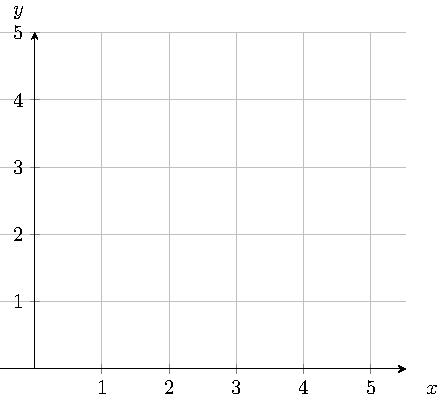
\includegraphics[scale=.8]{tikz-pictures/section-9.2-pic4-axes-for-projection-example.pdf}

\pagebreak 
\begin{ex}
    Still with $\vec{u}=\langle 4,1\rangle$ and $\vec{v}=\langle 3,4\rangle$, write $\vec{u}$ as a sum of vectors: one which is parallel to $\vec{v}$ and one which is perpendicular to $\vec{v}$.
\end{ex}
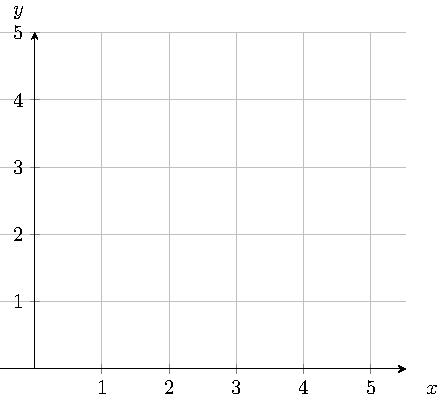
\includegraphics[scale=.8]{tikz-pictures/section-9.2-pic4-axes-for-projection-example.pdf}

The idea that we used in the above exercise works in general.\\
\begin{thm}[Orthogonal decomposition]
    For vectors $\vec{u}$ and $\vec{v}$ with $\vec{v}\ne\vec{0}$, we can write $\vec{u}$ as a sum of two vectors
    \[\vec{u}=\proj_{\vec{v}}(\vec{u})+\proj_{\perp\vec{v}}(\vec{u})\] where
    \begin{multicols}{2}
    \begin{itemize}
        \item $\displaystyle\proj_{\vec{v}}(\vec{u})$ is parallel to $\vec{v}$; and 
        \item $\displaystyle\proj_{\perp\vec{v}}(\vec{u})$ is orthogonal to $\vec{v}$.
    \end{itemize}\end{multicols}
    We call this an \emph{orthogonal decomposition} of $\vec{u}$ with respect to $\vec{v}$. In particular, we have
    \begin{multicols}{3}
    \begin{itemize}
        \item $\proj_{\vec{v}}(\vec{u}) = \phantom{ \dfrac{\vec{u}\dotp\vec{v}}{\vec{v}\dotp\vec{v}}\vec{v}}$
        \item $\proj_{\perp\vec{v}}(\vec{u}) = \phantom{\vec{u}-\proj_{\vec{v}}(\vec{u})}$
    \end{itemize}
    \end{multicols}
\end{thm}

\begin{defn}[Projection of $\vec{u}$ orthogonal to $\vec{v}$]
    The vector $\proj_{\perp\vec{v}}(\vec{u})$ is called the \emph{projection of $\vec{u}$ orthogonal to $\vec{v}$}.
\end{defn}

\noindent Application: We can use the orthogonal projection to compute the distance from a point to a line!

\begin{thm}[Distance from a point to a line]
    The distance from a point $P$ to a line which contains the points $Q$ and $R$ is\\
    \[
        \phantom{|\proj_{\perp\vec{v}}(\vec{u})|}
    \]
    \\
    where $\vec{u}=\vec{QP}$ and $\vec{v}=\vec{QR}$.
\end{thm}

\pagebreak 

\subsection{Physical interpretations of vectors}
Recall that the velocity of an object involves a direction and a speed. And the force applied by an object involves a direction and an amount of force. Thus, velocity and force can very naturally be represented by vectors.

The velocity vector of an object is the vector with direction and magnitude equal to, respectively, the object's direction of motion and the object's speed.

\begin{ex}
    A very wide river runs north, with water moving at a rate of 4 feet per second.
    
    A barracuda swims due north at a rate of 6 feet per second relative to the moving water. How fast, relative to the shore, is the barracuda moving?
\end{ex}

\vfill

\begin{ex}
    In the same river, a dolphin swims due east at a rate of 6 feet per second relative to the moving water. How fast, relative to the shore, is the dolphin moving? In what direction is the dolphin actually traveling?
\end{ex}
\vfill\vfill

